\section{Affine $n$-Space and Algebraic Sets}\label{section_1.2}

\begin{definition}
  Let $k$ be a field. We define \textbf{affine $n$-space} over $k$ to
  be the cartesian product
  \begin{equation*}
    \A^n(k)=\underbrace{k \times \dots \times k}_{n\text{--times}}
    = k^n
  \end{equation*}
  We call the elements of $A^n(k)$ \textbf{affine points} (or simply
  \textbf{points}). We call $\A^1(k)$ the \textbf{affine line} over
  $k$, and $\A^2(k)$ the \textbf{affine plane} over $k$.
\end{definition}

\begin{definition}
  Let $k$ be a field, and let $f(x_1, \dots, x_n) \in k[x_1, \dots,
  x_n]$. We call an affine point $P \in \A^n(k)$ a \textbf{root}, or a
  \textbf{zero} of $f(x_1, \dots, x_n)$ if $f(P)=0$; where
  $f(P)=f(a_1, \dots, a_n)$ whenever $P=(a_1, \dots, a_n)$. We define
  the \textbf{zero-locus} (or \textbf{locus}) of $f(x_1, \dots, x_n)$
  to be:
  \begin{equation*}
    V(f)=\{P \in \A^n(k) : f(P)=0\}
  \end{equation*}
  If $S \subseteq k[x_1, \dots, x_n]$ is any set of polynomials, then
  the \textbf{zero-locus} of $S$ is defined to be:
  \begin{equation*}
    V(S)=\{ P \in \A^n(k) : f(P)=0 \text{ for all } f \in S \}
  \end{equation*}
  and if $S=\{f_1, \dots, f_r\}$, we write $V(S)=V(f_1, \dots, f_r)$.
\end{definition}

\begin{proposition}\label{proposition_10.1.1}
  Let $k$ be a field, and let $S \subseteq k[x_1, \dots, x_n]$ be any
  set of polynomials over $k$. Then:
  \begin{equation*}
    V(S)=\bigcap_{f \in S}{V(f)}
  \end{equation*}
  moreover if $S$ is finite, then $V(S)$ is a finite intersection.
\end{proposition}
\begin{proof}
  By definition, if $P \in V(S)$ then for any $f \in S$, $f(P)=0$ so
  that $P \in \bigcap{V(S)}$. Conversley if $P \in \bigcap{V(f)}$,
  then $f(P)=0$ for all $f \in S$, so $P \in V(S)$.
\end{proof}

\begin{definition}
  Let $k$ be a field. We call a subset  $X \subseteq \A^n(k)$ an
  \textbf{affine algebraic set} (or just \textbf{algebraic set}) if
  $X=V(S)$ for some set of polynomials $S \subseteq k[x_1, \dots,
  x_n]$.
\end{definition}

\begin{proposition}\label{proposition_10.1.2}
  Let $k$ be a field. Then the following statements about affine
  algebraic sets are true:
  \begin{enumerate}
    \item[(1)] If $\af \subseteq k[x_1, \dots, x_n]$ is an ideal
      generated by some set $S$ of polynomials over $k$ then
      $V(\af)=V(S)$.

    \item[(2)] If $\{\af_\a\}$ is some non-empty colleection of ideals
      in $k[x_1, \dots, x_n]$, then:
      \begin{equation*}
        V\Big{(} \bigcup_{\a}{\af_\a} \Big{)}=\bigcap_{\a}{V(\af_\a)}
      \end{equation*}

    \item[(3)] If $\af \subseteq \bf$, then $V(\bf) \subseteq V(\af)$.

    \item[(4)] Let $f,g \in k[x_1, \dots, x_n]$. Then $V(fg)=V(f) \cup
      V(g)$. Moreover, if $\af, \bf $ are ideals, in $k[x_1, \dots,
      x_n]$, then:
      \begin{equation*}
        V(\af\bf)=V(\af) \cup V(\bf)
      \end{equation*}
      Indeed, finite unions of algebraic sets are algebraic.

    \item[(5)] $V(0)=\A^n(k)$ and $V(1)=\emptyset$. Moreover,
      $V(x_1-a_1, \dots, x_n-a_n)=\{(a_1, \dots, a_n)\}$ for any $a_1,
      \dots, a_n \in k$.
  \end{enumerate}
\end{proposition}
\begin{proof}
  Recall that since $k$ is a field, then $k[x_1, \dots, x_n]$ is
  Noetherian, and hence the ideals in $k[x_1, \dots, x_n]$ are
  finitely generated.
  \begin{enumerate}
    \item[(1)] Let $\af=(S)=(f_1, \dots, f_r)$, and let $P \in V(I)$.
      Then by definition, since $S \subseteq \af$, $f_i(P)=0$ for all
      $1 \leq i \leq r$ so that $P \in \bigcap_{i=1}^r{V(f_i)}=V(S)$.
      On the otherhand, let $P \in V(S)$ so that $f_i(P)=0$ for all $1
      \leq i \leq r$. Take $f \in \af$ so for some $g_1, \dots, g_n
      \in k[x_1, \dots, x_]$ we get
      \begin{equation*}
        f(P)=g_1(P)f_1(P)+\dots+g_r(P)f_r(P)=
        g_1(P)0+\dots+g_r(P)0=0
      \end{equation*}
      so $f(P)=0$ which pust $P \in V(\af)$

    \item[(2)] Take $\af=\bigcup{\af_\a}$ for some index $\a$. Let $P
      \in V(\af)$, so for any $f \in \af$ $f(P)=0$. But $f \in \af_\a$
      for some $\a$, hence $P \in V(\af_\a)$ for any $\a$. This puts
      $P  \in \bigcap{V(\af_\a)}$. Conversely, if $P \in
      \bigcap{V(\af_\a)}$, then $P \in V(\af_\a)$ for all $\a$, so
      that $P \in V(\af)$.

    \item[(3)] Let $\af \subseteq \bf$ be ideals in $k[x_1, \dots,
      x_n]$. Take $P \in V(\bf)$. Then for every $f \in \bf$,
      $f(P)=0$, by hypothesis, this makes $g(P)=0$ for every $g \in
      \af$. So $P \in V(\af)$.

    \item[(4)] Let $f,g \in k[x_1, \dots, x_n]$. Take $P \in V(fg)$.
      Then $fg(P)=f(P)g(P)=0$. Since $k$ is an integral domain, either
      $f(P)=0$ or $g(P)=0$, so $P \in V(f)$ or $P \in V(g)$.

      Conversely suppose that $P  \in V(f) \cup V(g)$. Then either
      $f(P)=0$ or $g(P)=0$. In either case we get $f(P)g(P)=fg(P)=0$
      so $P \in V(fg)$.

      Now, let $\af, \bf \subseteq k[x_1, \dots, x_n]$ be ideals, and
      let $P \in V(\af) \cup V(\bf)$. Then for any $f \in \af$ or for
      any $g \in \bf$ either $f(P)=0$ or $g(P)=0$. This puts $P \in
      V(\af\bf)$. Indeed if $\{\af_i\}_{i=1}^r$ is a family of ideals,
      and $\af=\prod_{i=1}^r{\af}$, then it follows from the above
      arguments that:
      \begin{equation*}
        V(\af)=\bigcup_{i=1}^r{V(\af_i)}
      \end{equation*}

    \item[(5)] Observe first that $V(0) \subseteq \A^n(k)$. Now let $P
      \in \A^n(k)$ having coordinates $P=(a_1, \dots, a_n)$. Then
      \begin{equation*}
        0(P)=\sum{0a_1^{d_1} \dots a_n^{d_n}}=0
      \end{equation*}
      so that $P \in V(0)$. Likewise, let $P \in V(1)$. Then $1(P)=0$.
      But also notice that:
      \begin{equation*}
        1(P)=1+\sum{0a_1^{d_1} \dots a_n^{d_n}}=1
      \end{equation*}
      which makes $1=0$ in $k$, which is impossible. Hence
      $V(1)=\0$.

      Lastly, let $P=(a_1, \dots, a_n)$. Then $P \in V(x_1-a_1, \dots,
      x_n-a_n)$ since $a_i-a_i=0$ for any $x_i-a_i$. Now, let $P \in
      V(x_1-a_1, \dots, x_n-a_n)$. Then for any $f \in (x_1-a_1,
      \dots, x_n-a_n)$ we get, letting $P=(b_1, \dots, b_n)$
      \begin{equation*}
        f(P)=(b_1-a_1)g_1(P)+\dots+(b_n-a_n)g_n(P)=0
      \end{equation*}
      which makes $b_i=a_i$ for all $1 \leq i \leq n$. This
      establishes that $V(x_1-a_1, \dots, x_n-a_n)=\{(a_1, \dots,
      a_n)\}$.
  \end{enumerate}
\end{proof}

\begin{example}\label{example_10.1}
  \begin{enumerate}
    \item[(1)] The following curves in figure \ref{figure_1.1} define
      algebraic sets over $\R$.
      \begin{figure}[h]
        \centering
        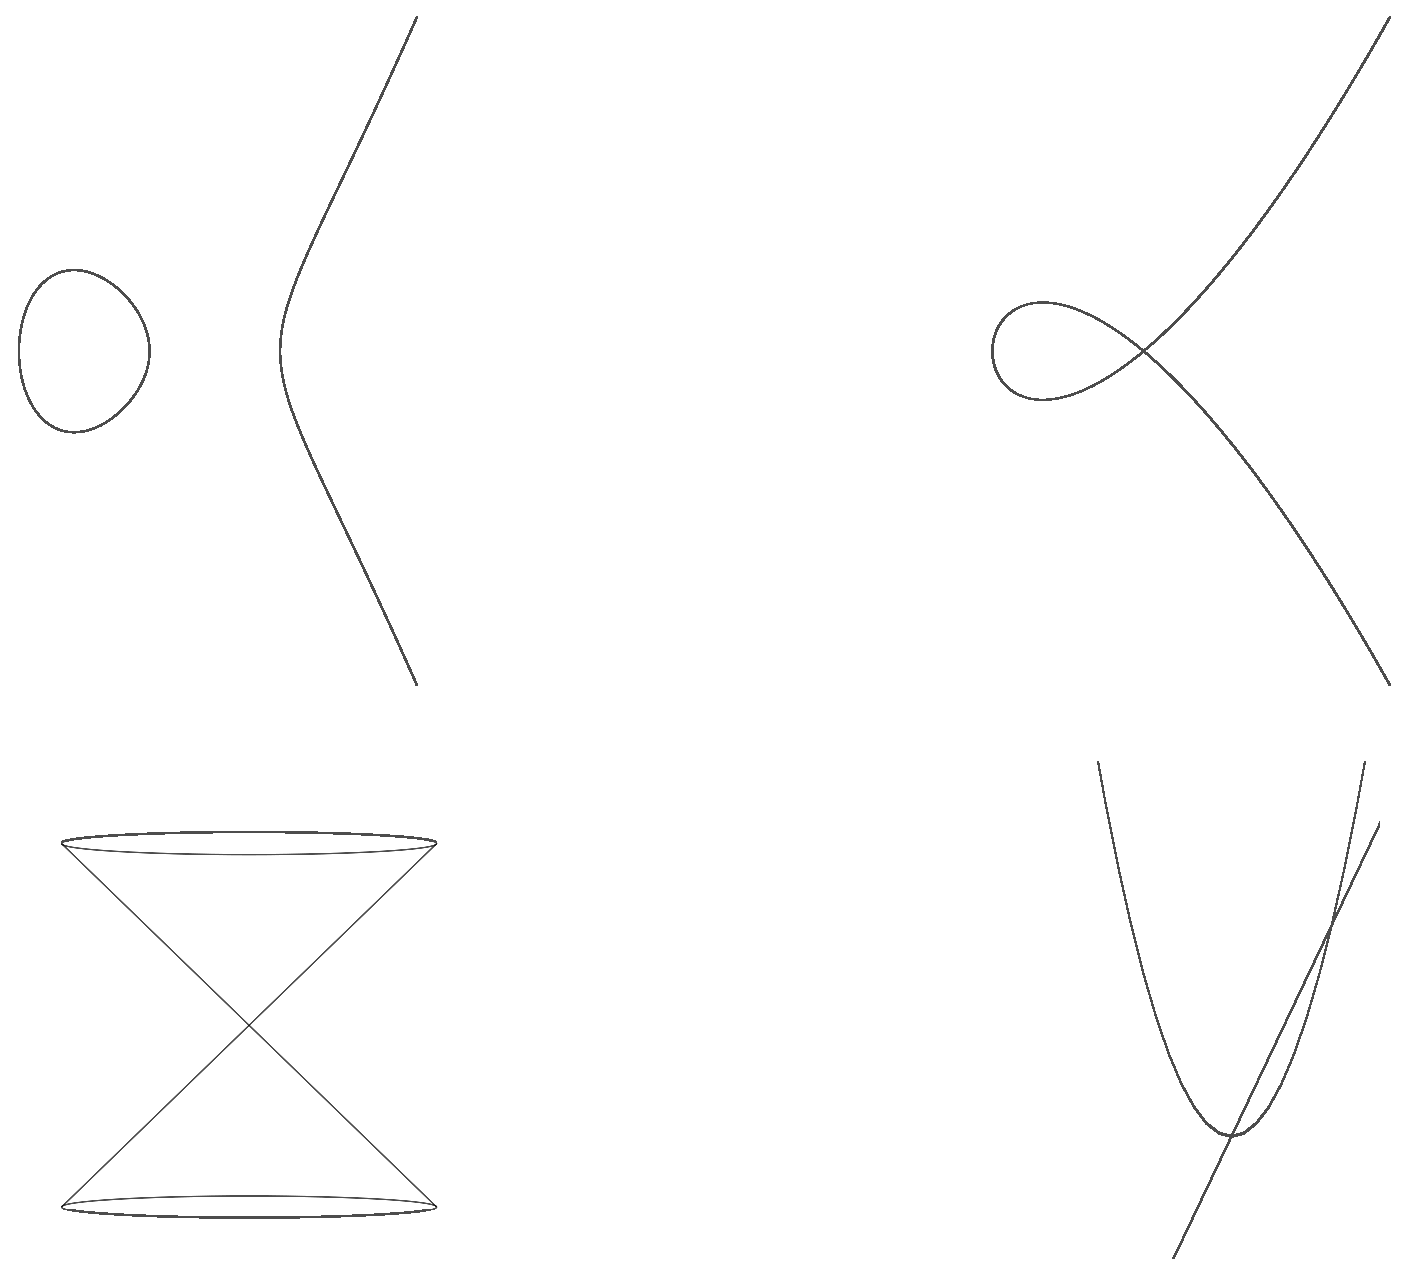
\includegraphics[scale=0.5]{parts/algebraic_curves/figures/Chapter1/hyperplanes.eps}
        \caption{Affine Algebraic Sets in $\A^2(\R)$ and $\A^3(\R)$.}
        \label{figure_1.1}
      \end{figure}

    \item[(2)] Let $k$ be any field, and let $X \subseteq \A^1(k)$ be
      an algebraic set. Then $X=V(S)$ for some set $S \subseteq k[x]$
      of polynomials. However, observe that for any $f(x) \in S$, with
      $\deg{f}=n$ that $f(x)$ has at most $n$ roots in $k$. Then
      $|V(f)| \leq n$. Now, since
      \begin{equation*}
        V(S) = \bigcap_{f \in S}{V(S)}
      \end{equation*}
      $|X|=|V(S)|$ is finite in $\A^1(k)$. Now also observe that
      $\A^1(k)=V(0)$. So the algebraic sets of $\A^1(k)$ are those
      finite point-sets, and $\A^1(k)$ itself.

    \item[(2)] Let $k$ be any field, and let $X \subseteq \A^n(k)$ be
      a finite point-set. Then $X=\{P_1, \dots, P_r\}$. Now let
      $P_i=(a_{i1}, \dots, a_{in})$. We have $V(x_1-a_{i1}, \dots,
      x_n-a_{in})=\{P_i\}$ so:
      \begin{equation*}
        X=\bigcup_{i=1}^r{V(x_1-a_{i1}, \dots, x_1-a_{in})}
      \end{equation*}
      which is an algebraic set by proposition
      \ref{proposition_10.1.2}.

    \item[(3)] Consider the finite field $\F_q$. Then the affine space
       $\A^n(\F_q)$ has exactly $q^n$ points. Hence if $X \subseteq
       \A^n(\F_q)$, then $|X| \leq q^n$ which makes $X$ a finite
       point-set, and hence it must be algebraic. Therefore every
       element of $\A^n(\F_q)$ is algebraic.

     \item[(4)] Consider $\Q[x]$, and for any $n \in \Z^+$ let $a_n
       \in \Q$ and take $f_n(x)=x-a_n$. Then $V(f_n)=\{a_n\}$ so
       $V(f_n)$ is algebraic. However
       \begin{equation*}
         \bigcup_{n=1}^\infty{V(f_i)}=\{a_n\}_{n=1}^\infty
       \end{equation*}
       is not algebraic. Indeed, let $V=\bigcup_{n=1}^\infty{V(f_i)}$.
       Then $V$ is infinite. Now suppose that $V=V(\af)$ for some
       ideal $\af$. Since $\Q[x]$ is a P.I.D., $\af=(f)$ for some
       polynomial of $f(x) \in \Q[x]$ $\deg{f}=n$. Then $f(x)$ has
       at-most $n$ roots in $\Q$ so that $|V| \leq n$. This
       contradicts that $V$ is infinite. Therefore $V$ cannot be
       algebraic.
  \end{enumerate}
\end{example}

\begin{example}\label{example_10.2}
  The following sets are algebraic.
  \begin{enumerate}
    \item[(1)] Consider $X=\{(t, t^2, t^3) \in \A^3(k) : t \in k\}$.
      Take $f(x,y,z)=x^3-z$ and $g(x,y,z)=x^2-y$. Then
      $f(t,t^2,t^3)=t^3-t^3=0$ and $g(t,t^2,t^3)=t^2-t^2=0$ so
      $X \subseteq V(f,g)$. On the other-hand if $P \in V(f,g)$ with
      $P=(a_1, a_2)$, then $f(P)=a_1^3-a_3=0$ and $g(P)=a_1^2-a_2=0$, so
      $P=(a_1, a_1^2, a_1^3)$. Which makes $V(f,g) \subseteq X$. We call
      the algebraic set
      \begin{equation*}
        V(x^3-z,x^2-y)=\{(t,t^2,t^3) \in \A^3(k): t \in k\}
      \end{equation*}
      the \textbf{twisted cubic} on $k$.

    \item[(2)] Let $X=\{(\cos{t}, \sin{t}) \in \R^2 : t \in \R\}$.
      Take $f(x,y)=x^2+y^2-1$. Then if $f(x,y)=0$ we get $x^2+y^2=1$
      which defines the unit circle in $\R^2$. Indeed,
      $X=V(x^2+y^2-1)$.

    \item[(3)] Let $X$ be the set of all points in $\R^2$ whose polar
      coordinates, of the form $(r, \th)$ satisfy $r=\sin{\th}$.
      Indeed, let $(x,y) \in X$. Then $x^2+y^2=r^2=\sin^2{\th}$.
      Define the $f(x,y)=x^2+y^2-\sin^2{\th}$. Then $X=V(f)$.

    \item[(4)] Let $k$ be any field, and choose $a,b \in k$. Define
      $f(x,y)=y-(ax+b)$. Then if $f(x,y)=0$ then $y=ax+b$. Conversely,
      if $P=(a_1, a_2)$ such that $a_1=\inv{a}(a_2-b)$ then observe
      that $f(P)=a_2-(a(\inv{a}(a_2-b))+b)=a_2-a_2=0$, so that
      \begin{equation*}
        V(y-(ax+b))=\{(a_1,a_2) \in \A^2(k) : a_1=\inv{a}(a_2-b)\}
      \end{equation*}
      Indeed, we have characterized all points for which $y=ax+b$.
      When $k=\R$, then $V(y-(ax+b))$ characterizes a line.
  \end{enumerate}
\end{example}

\begin{definition}
  Let $k$ be a field. We call the zero-locus of a non-constant
  polynomial $f(x_1, \dots, x_n) \in k[x_1, \dots, x_n]$ the
  \textbf{hypersurface} defined by $f(x_1, \dots, x_n)$. A
  hypersurface of degree $1$ is call a \textbf{hyperplane}. We call a
  hypersurface in $\A^2(k)$ an (\textbf{affine}) \textbf{plane curve}
  and we call a hyperplane in $\A^2(k)$ a \textbf{line}.
\end{definition}

\begin{theorem}\label{theorem_10.1.3}
  Let $k$ be any field, and let $C \subseteq \A^2(k)$ be an affine
  plane curve defined by a polynomial of degree $n$. If
  $L \subseteq \A^2(k)$ is a line such that $L \not\subseteq C$ then
  $L$ intersects $C$ at no more than $n$ points.
\end{theorem}
\begin{proof}
  Observe that if $L \subseteq C$ then $L \cap C=C$ and $L$ intersects
  $C$ at every point of  $C$.
  Now, by definition, since $L$ is a line, $L=V(y-(ax+b))$ for some
  $a,b \in k$. Now, let
  \begin{equation*}
    g(x)=f(x,ax+b)
  \end{equation*}
  in $k[x]$. Let $P \in L \cap C$ with $P=(x,y)$. Then $f(x,y)=0$ and
  $y-(ax+b)=0$ so that $f(x,ax+b)=0$ which puts $P \in V(g)$.
  Conversley, let $x \in V(g)$, then $g(x)=f(x,ax+b)=0$. Take $y=ax+b$
  for some $a,b \in k$. Then that we get the point $P=(x,y) \in L \cap C$.
  This makes $L \cap C=V(g)$. Since $V(g) \subseteq \A^1(k)$ and
  $\deg{g}=n$ we have that $V(g)$ contains no more than $n$ points.
\end{proof}

\begin{example}
  The following sets are not algebraic.
  \begin{enumerate}
    \item[(1)] Let $C=\{(x,y) \in \R^2 : y=\sin{x}\}$. Let $L$ be the
      line defined by $f(x,y)=y-\frac{1}{2}$. Then $L \not\subseteq
      C$, and $L$ intersects $C$ at infinitely many points.
  \end{enumerate}
\end{example}
